
\documentclass{article}
\usepackage[margin=1in]{geometry} 
\usepackage[french]{babel}
\usepackage[T1]{fontenc}
\usepackage[utf8]{inputenc}
\usepackage{amsmath,amsthm,amssymb,amsfonts, fancyhdr, color, comment, graphicx, environ}
\usepackage{xcolor}
\usepackage{mdframed}
\usepackage[shortlabels]{enumitem}
\usepackage{indentfirst}
\usepackage{hyperref}
\usepackage{lastpage}
\usepackage{listingsutf8}
\usepackage{ff++listings}

\renewcommand{\footrulewidth}{0.8pt}
\hypersetup{
    colorlinks=true,
    linkcolor=blue,
    filecolor=magenta,      
    urlcolor=blue,
}

\pagestyle{fancy}

\newenvironment{problem}[2][Etape]
    { \begin{mdframed}[backgroundcolor=gray!20] \textbf{#1 #2} \\}
    {  \end{mdframed}}


\newenvironment{solution}{\textbf{Réponse}}

\lhead{L. Gomes et F. Pollet}
\rhead{ES Elements finis} 
\chead{\textbf{Optimisation de l'épaisseur d'un pont}}
\lfoot{D. Ryckelynck, N. Spillane, P.-H. Tournier}
\cfoot{Mines Paris}
\rfoot{\thepage/\pageref*{LastPage}}

\begin{document}

    \title{\Large ES Elements Finis  \\[0.5cm]
        \bf\Large Optimisation de l'épaisseur d'une structure tridimensionnelle}
\author{\large Leticia Gomes\\Pollet Florent \ \\}
\date{\large\today}

\makeatletter
    \begin{titlepage}
        \begin{center}
	   { 
\includegraphics[width=12cm]{mp_logo.png}}
	   {\ \\ \ \\}
        \vbox{}\vspace{5cm}
            {\@title }\\[3cm] 
            {\@author}
            {\large \ \\ Encadrants: \bf David Ryckelynck, Nicole Spillane et Pierre-Henri Tournier\\ \ \\}
            {\@date\\}

        \end{center}
    \end{titlepage}

    \tableofcontents

    \clearpage
\makeatother%not necessary but looks fancy

    % rappel du problème ? reprendre photo du sujet
    % référence à la fin
    % appendix pour code ?

    \section{Présentation du problème}
    Intro intro sur des éléments finis, parler de l'utilité d'eux pour les calculs    
    Une application envisageable pour les calculs des éléments finis est l'optimisation d'épaisseur d'une structure tridimensionelle, ce qui est l'objectif de ce projet. La structure chosit pour cela est un pont dont nous avons cherché à minimiser l'épaisseur qui donne un déplacement vertical maximal de son centre de 10 cm. Celui-ce est dû à l'application d'une force constante à la surface horizontale supèrieure du pont. La géométrie de cette problème est tridimensionnelle et sa coupe verticale est montré dans la Figure 1. %referencier la figure
    \begin{center}
	{ 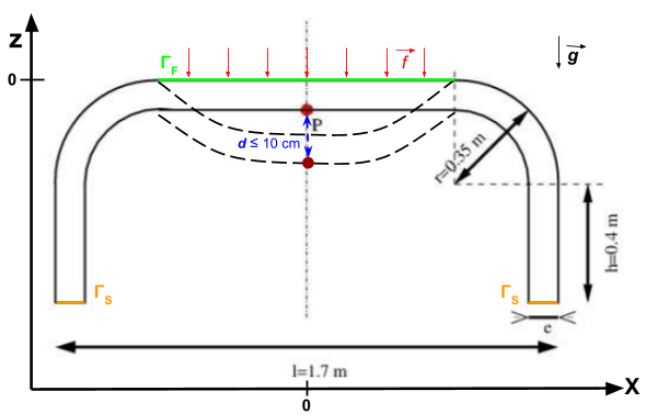
\includegraphics[width=12cm]{coupe_2D-schema.JPG}}
    % mettre la légende: Figure 1 - Coupe verticale de la géométrie du pont. Une force $f= - 5x10^8 N m^(-2)$ est appliquée à sa surface supérieure. Le déplacement maximale $d$ est montré en bleue. Le système est qui est soumis à la gravité $g$. Parler partie conditions limites ici!!!!!!!!!!! 
    La structure est considérée comme homogène avec les extrémités inferiures fixes et une épaisseur $p = 0,5 m$. Les donnés fournis pour ce système sont:
    \begin{itemize}
    \item **Module d'Young :** $E = 2,1x10^11 N m^(-2)$
    \item **Coefficient de Poisson :** $\nu = 0,3$
    \item **Masse Volumique :** $\rho = 7800 kg m^(-3)$
    \item **Force imposée sur le bord supérieur :** $f= - 5x10^8 N m^(-2)$
    \end{itemize}
    Nous avons divisé l'execution de ce projet dans trois parties :
    1. Établissement de la formulation variationelle pour ce problème ;
    2. Résolution à épaisseur fixée : nous avons écrit un programme avec la langage FreeFem++ pour résoudre le système à épaisseur fixe $e = 0,1 m$, avec une maille itialement bidimentionelle qui a été changé à tridimensionelle avec la fonction $buildlayers$. Nous avons étudié la différence entre des solutions calculés pour la pièce et pour son moitié et aussi la précision du résultat en variant le maillage.
    3. Optimisation de l'épaisseur : 
    	a. Approximation graphique : nous avons analysé la rélation entre l'épaisseur et le déplacement afin de trouver un intervalle où le déplacement est inférieur ou égal à 10 cm.
	b. Raffinement de la solution : nous avons utilisé la méthode de dichotomie pour résoudre le système.
    \section{Formulation variationnelle}

    \begin{problem}{1}
    Mise sous équation
    \end{problem}
    
    \begin{solution}    
    Blabla
    \end{solution}

    \section{Résolution à épaisseur fixée}

    \section{Optimisation de l'épaisseur}

    \subsection{Approximation graphique}
    \subsection{Raffinement de la solution}
    
    \clearpage
    \appendix
    \section {Code source}

    Disponible sur ...

    \lstinputlisting[language=FreeFem]{simulation-v2.edp}


    %code + lien github
    
\end{document}
